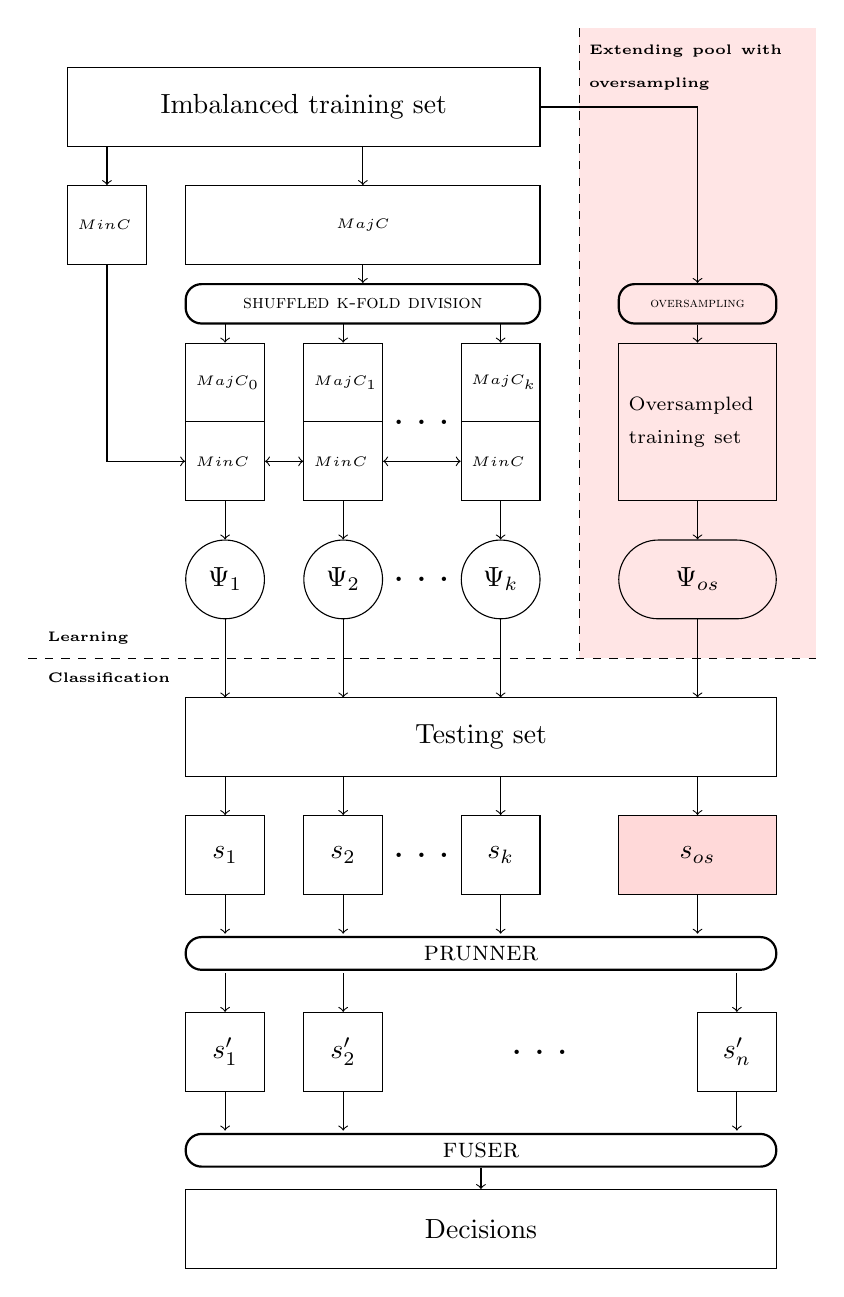
\begin{tikzpicture}%[font=\sffamily\small]
\tikzset{el/.style={draw, rectangle, minimum width = 1cm, minimum height=1cm}}

%\draw[step=.5cm,gray!30!white,very thin] (-4,-15) grid (7,1.5);

\node[rectangle, fill=red!10!white, minimum width=3cm, minimum height=8cm]
 at (5,-3) {};

% Original training set with division
\node[el, minimum width=6cm](its) at (0,0) {Imbalanced training set};
\node[el, text width=.75cm] (minc) at (-2.5, -1.5) {\tiny $MinC$};
\node[el, minimum width = 4.5cm] (majc) at (.75, -1.5) {\tiny $MajC$};

% Pre-methods
\node[el, thick, minimum width = 4.5cm, minimum height = .5cm, rounded corners=2mm] (kfold) at (.75, -2.5)
{\scriptsize \textsc{shuffled k-fold division}};
\node[el, thick, minimum width = 2cm, minimum height = .5cm, rounded corners=2mm] (oversampling) at (5, -2.5)
{\tiny \textsc{oversampling}};

% Processed training sets
\node[el, text width=.75cm] (majc0) at (-1, -3.5) {\tiny$MajC_0$};
\node[el, text width=.75cm] (majc1) at (.5, -3.5) {\tiny$MajC_1$};
\node[el, text width=.75cm] (majck) at (2.5, -3.5) {\tiny$MajC_k$};
\node[el, text width=.75cm] (minc0) at (-1, -4.5) {\tiny$MinC$};
\node[el, text width=.75cm] (minc1) at (.5, -4.5) {\tiny$MinC$};
\node[el, text width=.75cm] (minck) at (2.5, -4.5) {\tiny$MinC$};
\node[text width = 1cm] at (1.65,-4)
{\bfseries . . .};


\node[el, minimum width = 2cm, minimum height=2cm, text width=1.75cm] (osts) at (5, -4)
{\scriptsize Oversampled training set};

% Member classifiers
\node[el, rounded corners=5mm] (c0) at (-1, -6) {$\Psi_1$};
\node[el, rounded corners=5mm] (c1) at (.5, -6) {$\Psi_2$};
\node[el, rounded corners=5mm] (ck) at (2.5, -6) {$\Psi_k$};
\node[el, minimum width=2cm, rounded corners=5mm] (co) at (5, -6) {$\Psi_{os}$};

\node[text width = 1cm] at (1.65,-6)
{\bfseries . . .};


% Testing
\node[el, minimum width=7.5cm](testset) at (2.25,-8) {Testing set};

\node[el] (s0) at (-1, -9.5) {$s_1$};
\node[el] (s1) at (.5, -9.5) {$s_2$};
\node[el] (sk) at (2.5, -9.5) {$s_k$};
\node[el, minimum width=2cm, fill=red!15!white] (so) at (5, -9.5) {$s_{os}$};
\node[text width = 1cm] at (1.65,-9.5)
{\bfseries . . .};



\node[el, minimum width=7.5cm, minimum height = .5, thick, rounded corners=2mm](pruner) at (2.25,-10.75)
{\textsc{prunner}};

\node[el] (s_0) at (-1, -12) {$s'_1$};
\node[el] (s_1) at (.5, -12) {$s'_2$};
\node[el] (s_n) at (5.5, -12) {$s'_n$};
\node[text width = 1cm] at (3.15,-12)
{\bfseries . . .};


\node[el, minimum width=7.5cm, minimum height = .5, thick, rounded corners=2mm](fuser) at (2.25,-13.25)
{\textsc{fuser}};


\node[el, minimum width=7.5cm](dec) at (2.25,-14.25)
{Decisions};


% Lines and sections
\draw [dashed] (3.5,1) -- (3.5,-7);
\node[text width = 2.75cm] at (5,.5)
{\tiny \bfseries Extending pool with oversampling};
\node[text width = 2cm] at (-2.25,-6.75)
{\tiny \bfseries Learning};
\node[text width = 2cm] at (-2.25,-7.25)
{\tiny \bfseries Classification};

\draw [dashed] (-3.5,-7) -- (6.5,-7);

% Connections
\draw[->] (its) -| (oversampling);
\draw[->] (-2.5,-.5) -- (minc);
\draw[->] (.75,-.5) -- (majc);
\draw[->] (majc) -- (kfold);

\draw[->] (-1,-2.75) -- (majc0);
\draw[->] (.5,-2.75) -- (majc1);
\draw[->] (2.5,-2.75) -- (majck);

\draw[->] (minc.south) |- (minc0.west);
\draw[<->] (minc0) -- (minc1);
\draw[<->] (minc1) -- (minck);


\draw[->] (oversampling) -- (osts);

\draw[->] (minc0) -- (c0);
\draw[->] (minc1) -- (c1);
\draw[->] (minck) -- (ck);
\draw[->] (osts) -- (co);

\draw[->] (c0) -- (-1,-7.5);
\draw[->] (c1) -- (.5,-7.5);
\draw[->] (ck) -- (2.5,-7.5);
\draw[->] (co) -- (5,-7.5);

\draw[->] (-1,-8.5) -- (s0);
\draw[->] (.5,-8.5) -- (s1);
\draw[->] (2.5,-8.5) -- (sk);
\draw[->] (5,-8.5) -- (so);

\draw[->] (s0) -- (-1,-10.5);
\draw[->] (s1) -- (.5,-10.5);
\draw[->] (sk) -- (2.5,-10.5);
\draw[->] (so) -- (5,-10.5);

\draw[->] (-1,-11) -- (s_0);
\draw[->] (.5,-11) -- (s_1);
\draw[->] (5.5,-11) -- (s_n);


\draw[->] (s_0) -- (-1,-13);
\draw[->] (s_1) -- (.5,-13);
\draw[->] (s_n) -- (5.5,-13);

\draw[->] (fuser) -- (dec);



\end{tikzpicture}
